\documentclass[12pt,
    a4paper,
    headinclude,
    footinclude]{scrreprt}

    %plainfootsepline

\usepackage{blindtext}
\usepackage[utf8]{inputenc}
\usepackage{setspace}
\usepackage[ngerman]{babel}
\usepackage[ngerman, num]{isodate}
\usepackage[left=3cm,right=2cm,top=2.8cm,bottom=2.4cm]{geometry}

\usepackage[style=numeric]{biblatex}
\usepackage[babel,german=guillemets]{csquotes}

\usepackage{float}

\usepackage{graphicx}
\usepackage{tabularx}
\usepackage{caption}

\usepackage{listings}
\usepackage{color}
\renewcommand{\lstlistingname}{Auflistung}
\renewcommand{\lstlistlistingname}{Auflistungsverzeichnis}
\definecolor{hellgrau}{rgb}{.95,.95,.95}
\definecolor{grau}{rgb}{.9,.9,.9}
\lstset{
	%backgroundcolor=\color{hellgrau},
	%backgroundcolor=\color{blue}
	%basicstyle=\scriptsize\ttfamily,
	%keywordstyle=\bfseries\ttfamily\color{orange},
	%stringstyle=\color{green}\ttfamily,
	%commentstyle=\color{middlegray}\ttfamily,
	%emph={square}, 
	%emphstyle=\color{blue}\texttt,
	%emph={[2]root,base},
	%emphstyle={[2]\color{yac}\texttt},
	showstringspaces=false,
	%flexiblecolumns=false,
	tabsize=1,
	numbers=left,
	%numberstyle=\tiny,
	numberblanklines=false,
	stepnumber=1,
	%numbersep=0pt,
	xleftmargin=20pt,
	frame=l,
	framesep=4.5mm,
	framexleftmargin=2.5mm,
	fillcolor=\color{grau},
	rulecolor=\color{grau},
	%numberstyle=\normalfont\tiny\color{numbercolor}
}

\usepackage{wrapfig}

\bibliography{res33.bib} 


\AtBeginDocument{\setlength{\glslistdottedwidth}{.15\columnwidth}}
\usepackage[acronyms,style=listdotted,shortcuts,translate=babel,toc]{glossaries}
%\GlsSetXdyLanguage{german}                         % Deutsche Spracheinstellung (nicht ngerman!) 
%\GlsSetXdyCodePage{duden-utf8}                     % Deutsche Codierung 
%\newglossarystyle{glosstil}{                     % neuer Stil mit Namen
%	\glossarystyle{listdotted}                           % basierent auf Stil long
%	\renewenvironment{theglossary}
%	{\begin{longtable}
%			{@{}p{0.1\textwidth} p{0.8\textwidth}}}   % einstellen der Spaltenbreiten
%		{\end{longtable}}
%	\renewcommand*{\glsgroupskip}{}               % keine Gruppenumbrüche
%} 

%\renewcommand*{\glsgroupskip}{}
%\makeglossaries
% \newacronym{TCP}{TCP}{Transmission Control Protocol}
% \newacronym{FTP}{FTP}{File Transfer Protocol}
% \newacronym{IP}{IP}{Internet Protocol}
% \newacronym{DNS}{DNS}{Domain Name Server}
% \newacronym{WWW}{WWW}{World Wide Web}
% \newacronym{HTTP}{HTTP}{Hypertex Transfer Protocol}
% \newacronym{HTTPS}{HTTPS}{Hypertex Transfer Protocol Secure}
% \newacronym{HTML}{HTML}{Hypertex Markup Language}
% \newacronym{XML}{XML}{Extensible Markup Language}
% \newacronym{WS}{WS}{WebSocket}
% \newacronym{ASCII}{ASCII}{American Standard Code for Information Interchange}
% \newacronym{UTF-8}{UTF-8}{8-Bit Universal Character Set Transformation Format}
%\usepackage{etoolbox}

%\newacronym{}{}{}

%\usepackage{fontspec}
%\setmainfont{Times New Roman}
%\usepackage[T1]{fontenc}
%\newcommand{\changefont}[3]{
%\fontfamily{#1} \fontseries{#2} \fontshape{#3} \selectfont}

%\renewcommand{\chapterpagestyle}{scrheadings}


%kopf und fusszeile
%\usepackage[headsepline]{scrpage2}
%\pagestyle{scrheadings} 
%\setlength{\footskip}{8mm}
%\clearscrheadings
%\ihead{\leftmark}
%\ohead{\rightmark}
%\automark[section]{chapter}
%\cfoot{\pagemark}
%kopf und fusszeile

%Schriftart sfffamily serifenlos
\setkomafont{pageheadfoot}{\normalfont\rmfamily\bfseries}

\setkomafont{chapterentry}{\normalfont\rmfamily\bfseries}
%\setkomafont{sectionentry}{\normalfont\rmfamily}

\setkomafont{chapter}{\huge\normalfont\rmfamily\bfseries}
\setkomafont{section}{\Large\normalfont\rmfamily\bfseries}
%Schriftart



\DefineBibliographyStrings{ngerman}{%
	bibliography={Literaturverzeichnis}% NICHT references
}


\author{Martin Braun}
\title{Redfish}

\begin{document}
	\onehalfspacing
	\monthyearsepgerman{\,}{\,}
	\setcounter{tocdepth}{2}
	

	
	\begin{titlepage}
	
		\begin{center}
			~\\[2cm]
			Berufsakademie Sachsen \\
			Staatliche Studienakadamie Leipzig \\
			Studiengang Informatik \\
           	Evolutionäre Algorithmen\\ [2.4cm]
           
			\begin{Large}
			    \textbf{Binäre und reelle Kodierung im Vergleich bei der näherungsweisen Berechnung des globalen Minimums der Griewank-Funktion} \\[2.4cm]
			\end{Large}
			
			\doublespacing


		\end{center}
		\onehalfspacing
		\begin{tabbing}
			Eingereicht von: \= ~ \= ~ \= ~ \= Georg Andrássy \hspace*{3cm} Matrikelnr: 5000593  \\
			\> \> \> \> Martin Braun \hspace*{3.4cm} Matrikelnr: 5000562 \\
			\\

		\end{tabbing}
		\vspace*{\fill}
		Leipzig, \today
		
	\end{titlepage}
    
    %Inhaltsverzeichnis
%    \pagenumbering{Roman}
%    \tableofcontents 	
    \clearpage
    %Inhaltsverzeichnis
        
    \pagenumbering{arabic}
    \setcounter{page}{2}
    
\section*{1. Einführung}	\onehalfspacing

Zur näherungsweisen Berechnung des globalen Minimums der Griewank-Funktion: \[f(x) = 1 +  \sum_{i=1}^n \frac{x_i^{2}}{400n} -  \prod \limits_{i=1}^n cos \left(\frac{x_i}{\sqrt{i}}\right)\] wird ein evolutionärer Algorithmus eingesetzt. Dieser Algorithmus wird vor allem im Hinblick auf den Einfluss  unterschiedlicher Kodierungsarten sowie stabiler und wachsender Populationsgrößen auf den Fitnesswert der Individuen untersucht. Zusätzlich wird die Differenz zwischen dem besten und dem schlechtesten Individuum in der Population als Maß der Streuung betrachtet. Die Minimierung der Griewank-Funktion wird für drei verschiedene n (n=5, 20, 50) im Wertebereich von -512 bis 511 getestet:




\section*{2. Umsetzung}


Für die Umsetzung wird folgender Algorithmus verwendet:

\begin{enumerate}
	\item Erzeugung der Startpopulation 
	\begin{itemize}
		\item fixe Ausgangspopulation mit X Anfangsindividuen
	\end{itemize}
	\item Elternselektion
		\begin{itemize}
		\item Anzahl Elternpaar = e mit zufälliger Selektion
		\item e wachsend bzw. stabil
	\end{itemize}
	\item Rekombination
		\begin{itemize}
		\item Reelle Kodierung: intermediäre Rekombination
		\item Binärkodierung: Ein-Punkt- und Zwei-Punkt-Rekombination (Zwei-Punkt: Mittelteil austauschen)
	\end{itemize}
	\item Mutation
		\begin{itemize}
		\item Mutationswahrscheinlichkeit M [0,1]
		\item von jedem Individuum soll zufällig ein Gen ausgewählt werden
		\item für Mutation eines Gens Zufallszahl z [0,1] ermitteln
		\item Reelle Kodierung: wenn z $<$ M, dann mutiere: addiere zum gewählten Allel einen festen Wert W
		\item Binärkodierung: zufällig von dem gewählten Binär-Allel ein Bit auswählen, wenn z $<$ M, dann switche Bit von 0 zu 1 bzw. 1 zu 0
	\end{itemize} 
	\item Umweltselektion
		\begin{itemize}
		\item aus Eltern + Kindern soll neue Population gewählt werden 
		\item zuerst die besten A Individuen nehmen (deterministische Selektion) Gesamtpopulation soll wachsen (A wächst linear von Generation zu Generation um +1 an)
		\item dann aus Rest zufällig B Individuen auswählen
	\end{itemize}
	\item gehe zu Punkt 2 bis Abbruchkriterium K erreicht
\end{enumerate}

\begin{table}[h]
	\centering
	\caption*{Verwendete Parameter}
	\begin{tabularx}{14cm}{|p{9cm}|X|}
		\hline
		$Parameter$ & $Wert$ \\
		\hline
		\hline
		Größe der Startpopulation X Individuen& 10  \\
				\hline
		Anzahl der Elternpaare e & 10 (+1 pro Zyklus)  \\
				\hline
		Rekombinationswahrscheinlichkeit& 0.9 \\
				\hline
		Mutationswahrscheinlichkeit M & 0.1 \\
				\hline
		reeller Mutationswert W& +5.0  \\
				\hline
		Auswahl bester Individuen a& 10 (+1 pro Zyklus) \\
		\hline
		Auswahl zufällige Umweltselektion B& 3 \\
		\hline
		Abbruchkriterium K Zyklen & 1500\\
		\hline
	\end{tabularx}
\end{table}


	
\section*{3. Ergebnisse und Interpretation}	

Die Ergebnisse wurden für vier verschiedene Aspekte ermittelt (Mittelwerte von 100 Versuchen, Abbruch nach 500 Zyklen):

\begin{enumerate}
	\item Vergleich zwischen Reeller und Binärer Kodierung (1-Punkt- und 2-Punkt-Rekombination)
    \item Vergleich zwischen stabiler und wachsender Population
    \item Vergleich zwischen verschiedener Anzahl an Genen (für n = 5, 20, 50)
    \item Vergleich zwischen Streuung innerhalb der Kodierungsarten 
\end{enumerate}

Beim Vergleich der Kodierungsarten in Abbildung 1 fällt auf, dass die beiden binären Kodierungsarten bessere Fitnesswerte bringen. Innerhalb der Binärkodierung bringt zusätzlich die Eins-Punkt-Rekombinationsmethode noch einen schnelleren Abfall zum globalen Minimum. 

\begin{figure}[H]
	\centering
	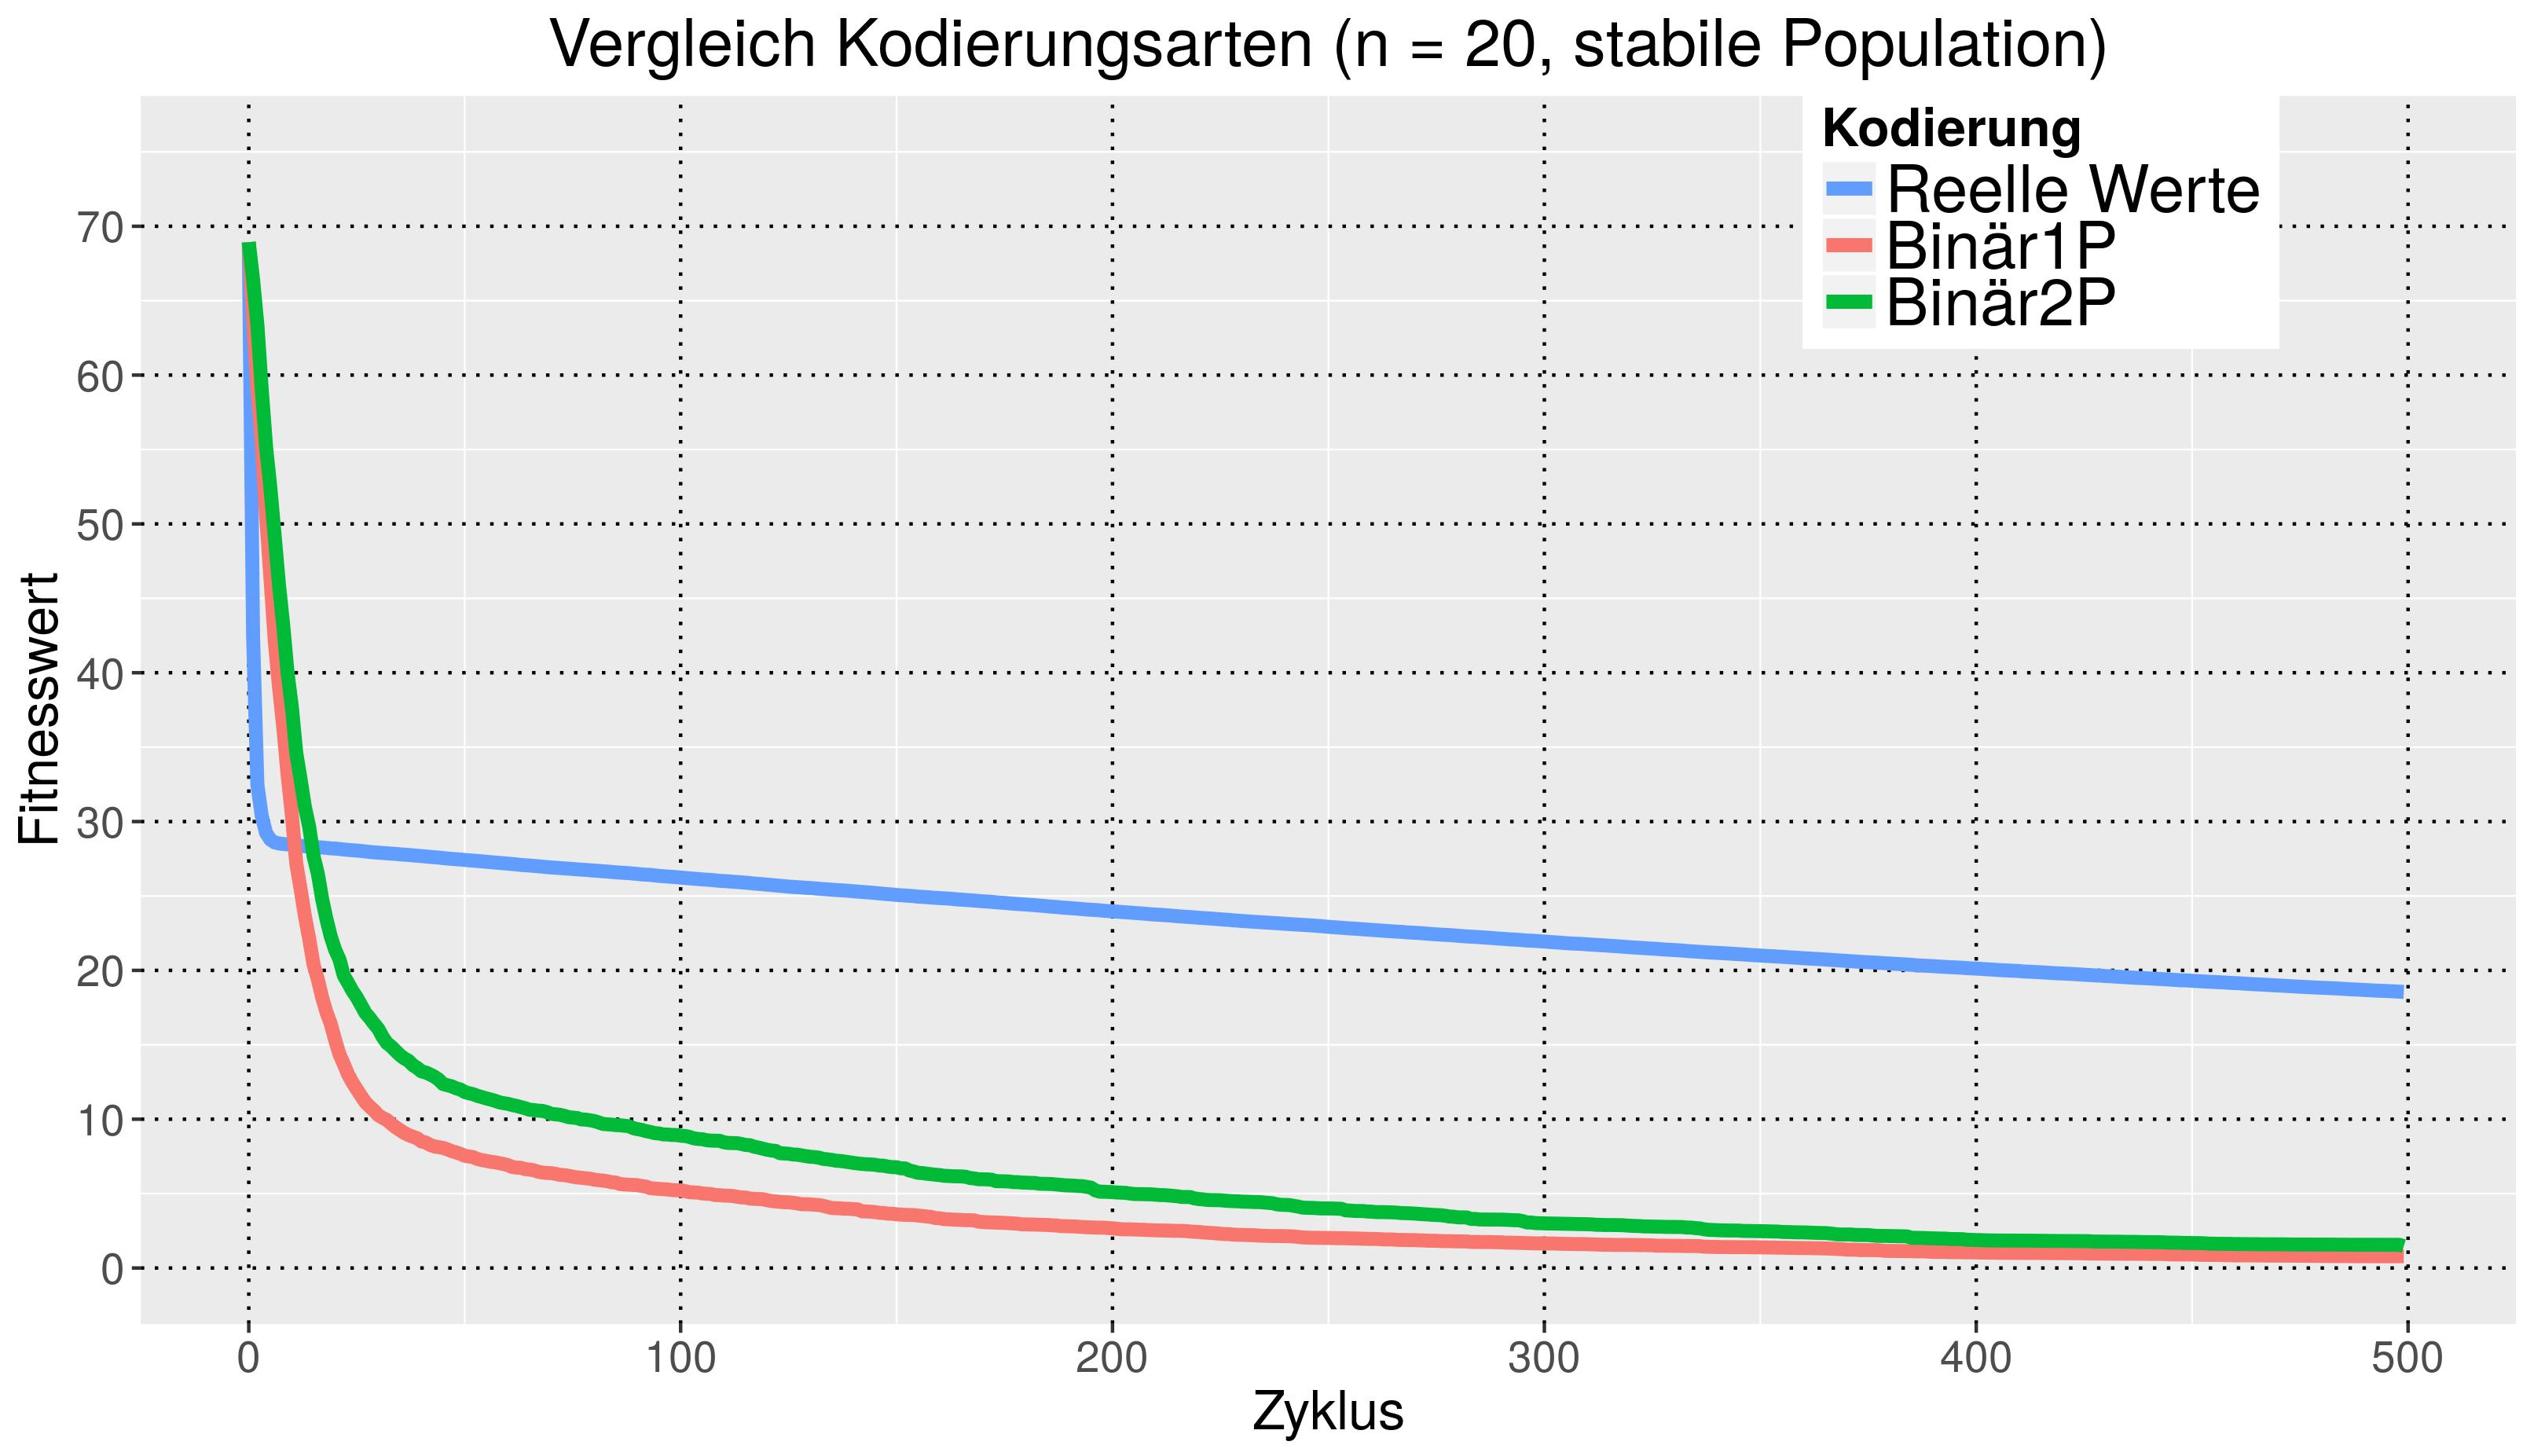
\includegraphics[width=0.7\textwidth]{../abb1_n20_stable.jpeg} 
	
	\caption*{Abb.1: Kodierungen im Vergleich bei n=20 (stabile Population)} 
	\label{InputOutput}
\end{figure}

Nach Abbildung 2 für n = 50 liefert der Algorithmus mit wachsender Population ein besseres Ergebnis als mit stabiler Population.

\begin{figure}[H]
	\centering
	\begin{minipage}[b]{0.45\textwidth}
		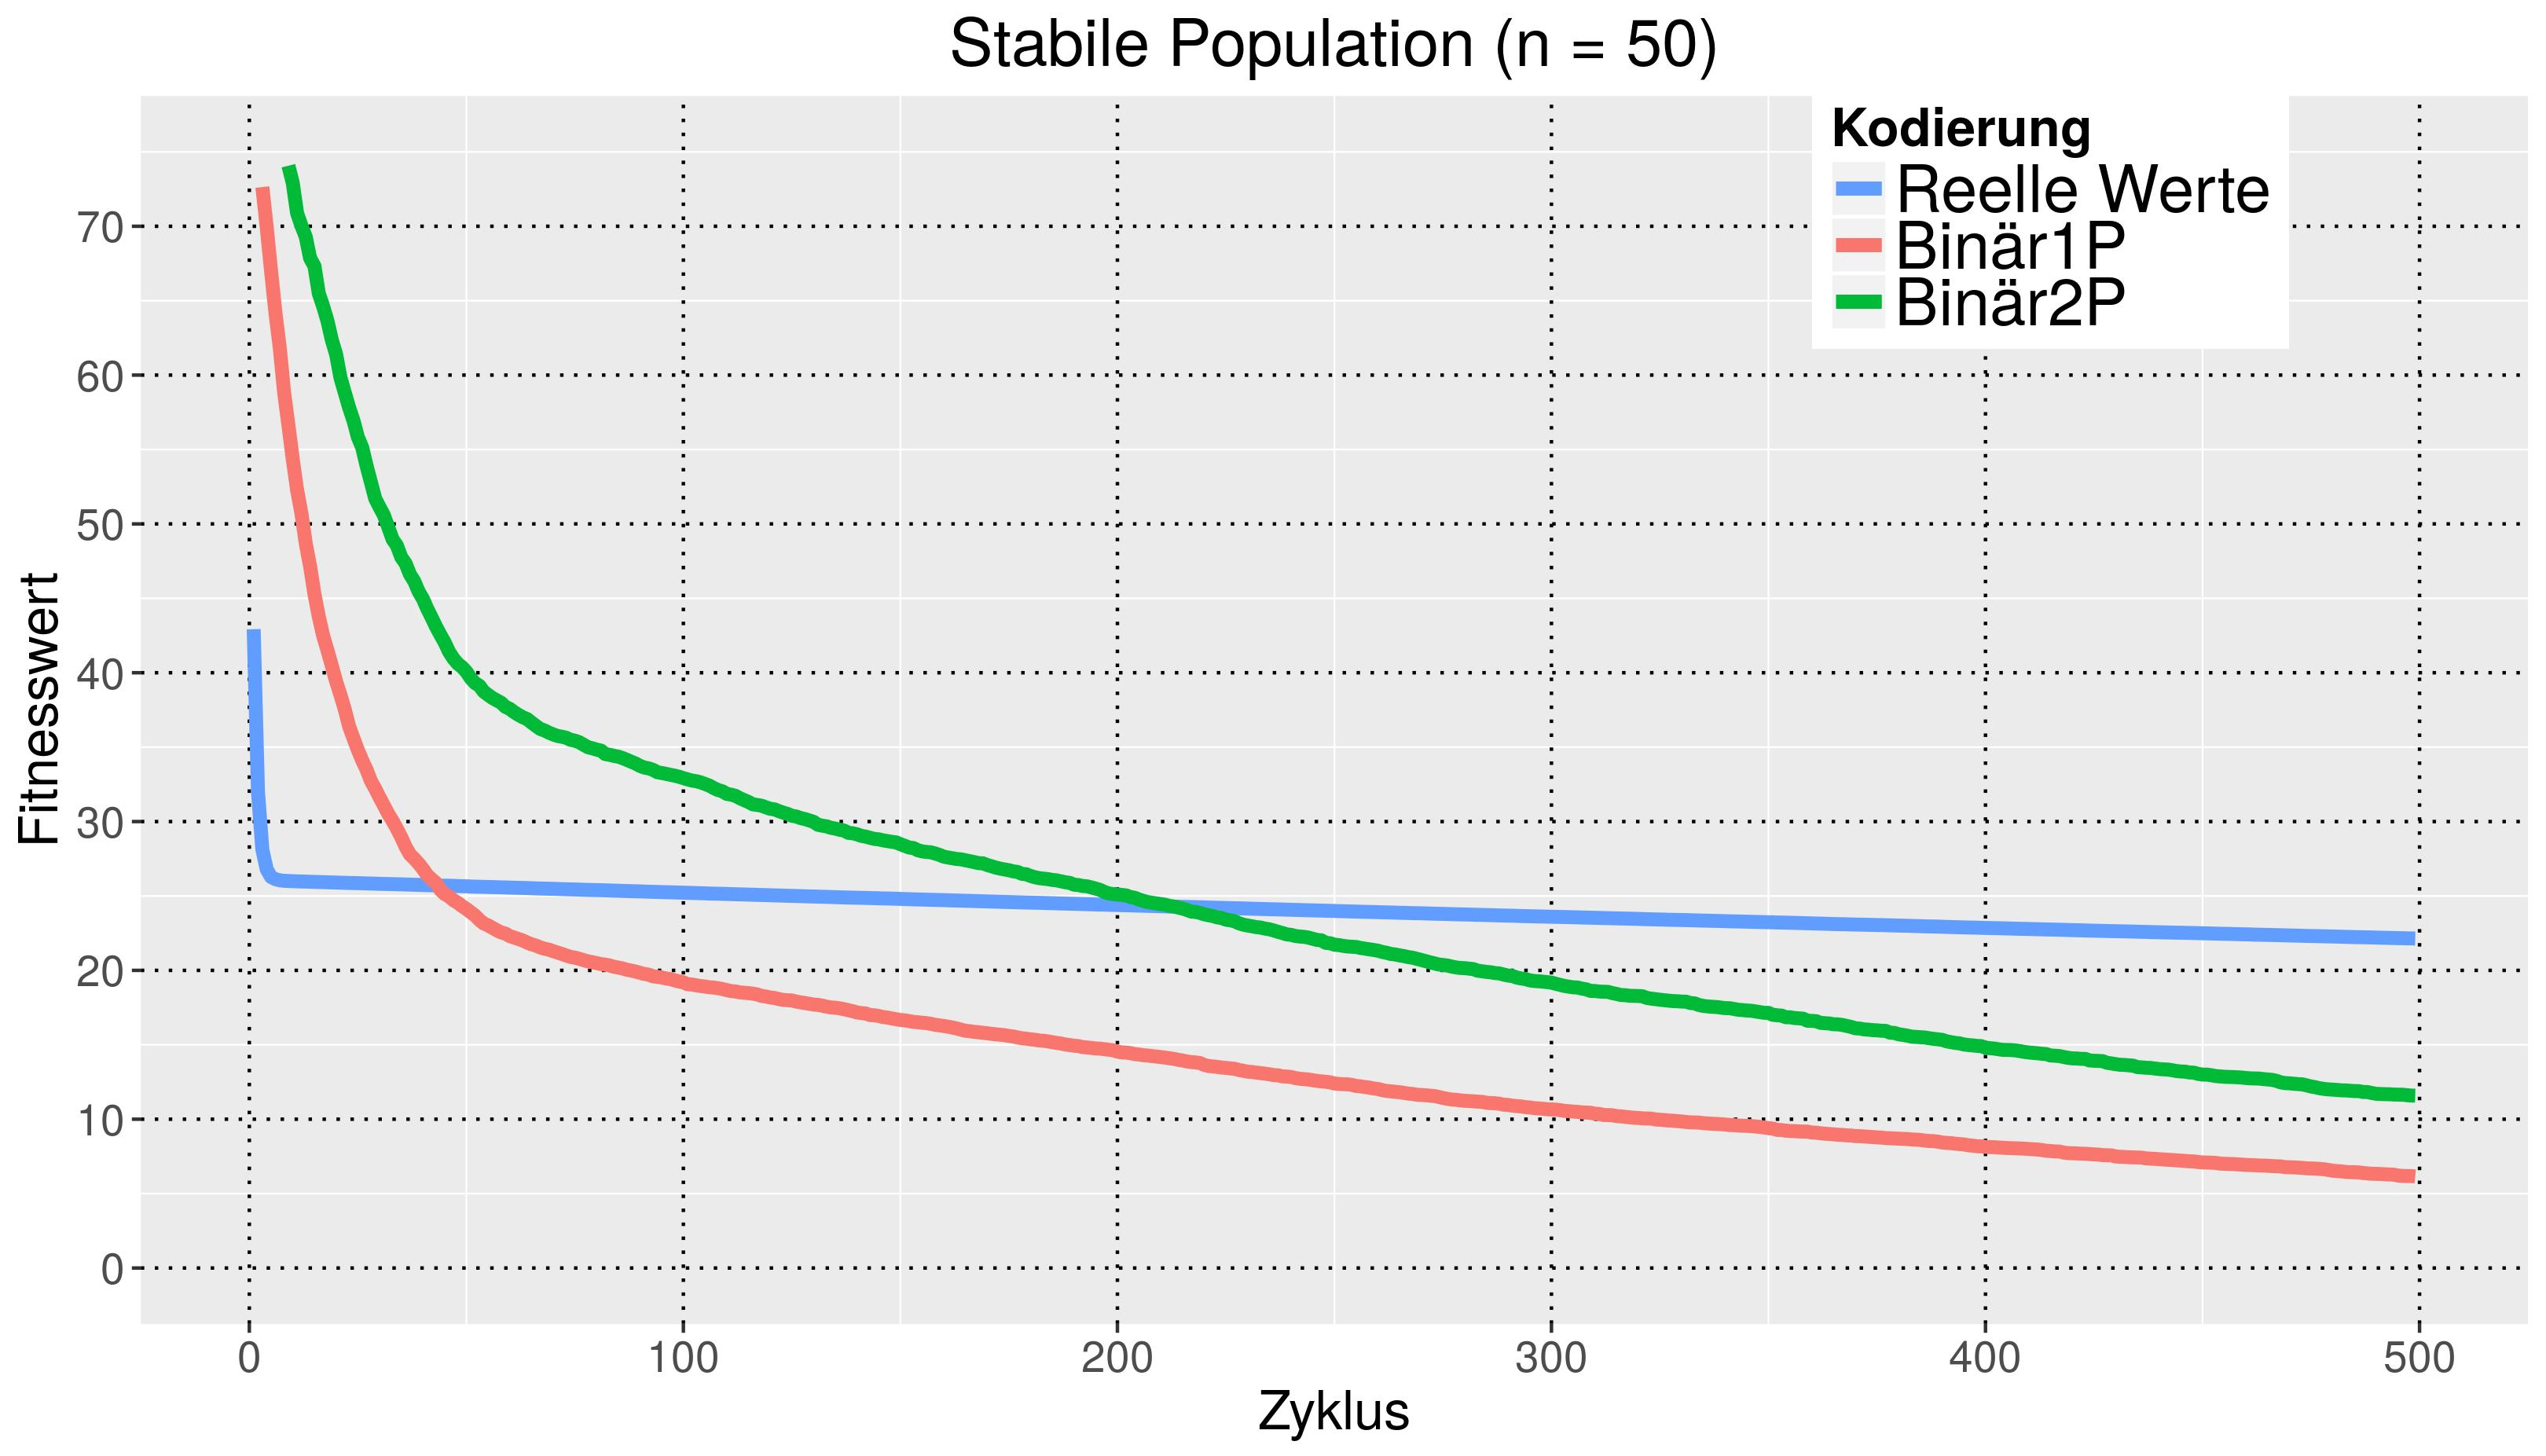
\includegraphics[width=\textwidth]{../abb2_stable.jpeg}
	\end{minipage}
	\hfill
	\begin{minipage}[b]{0.45\textwidth}
		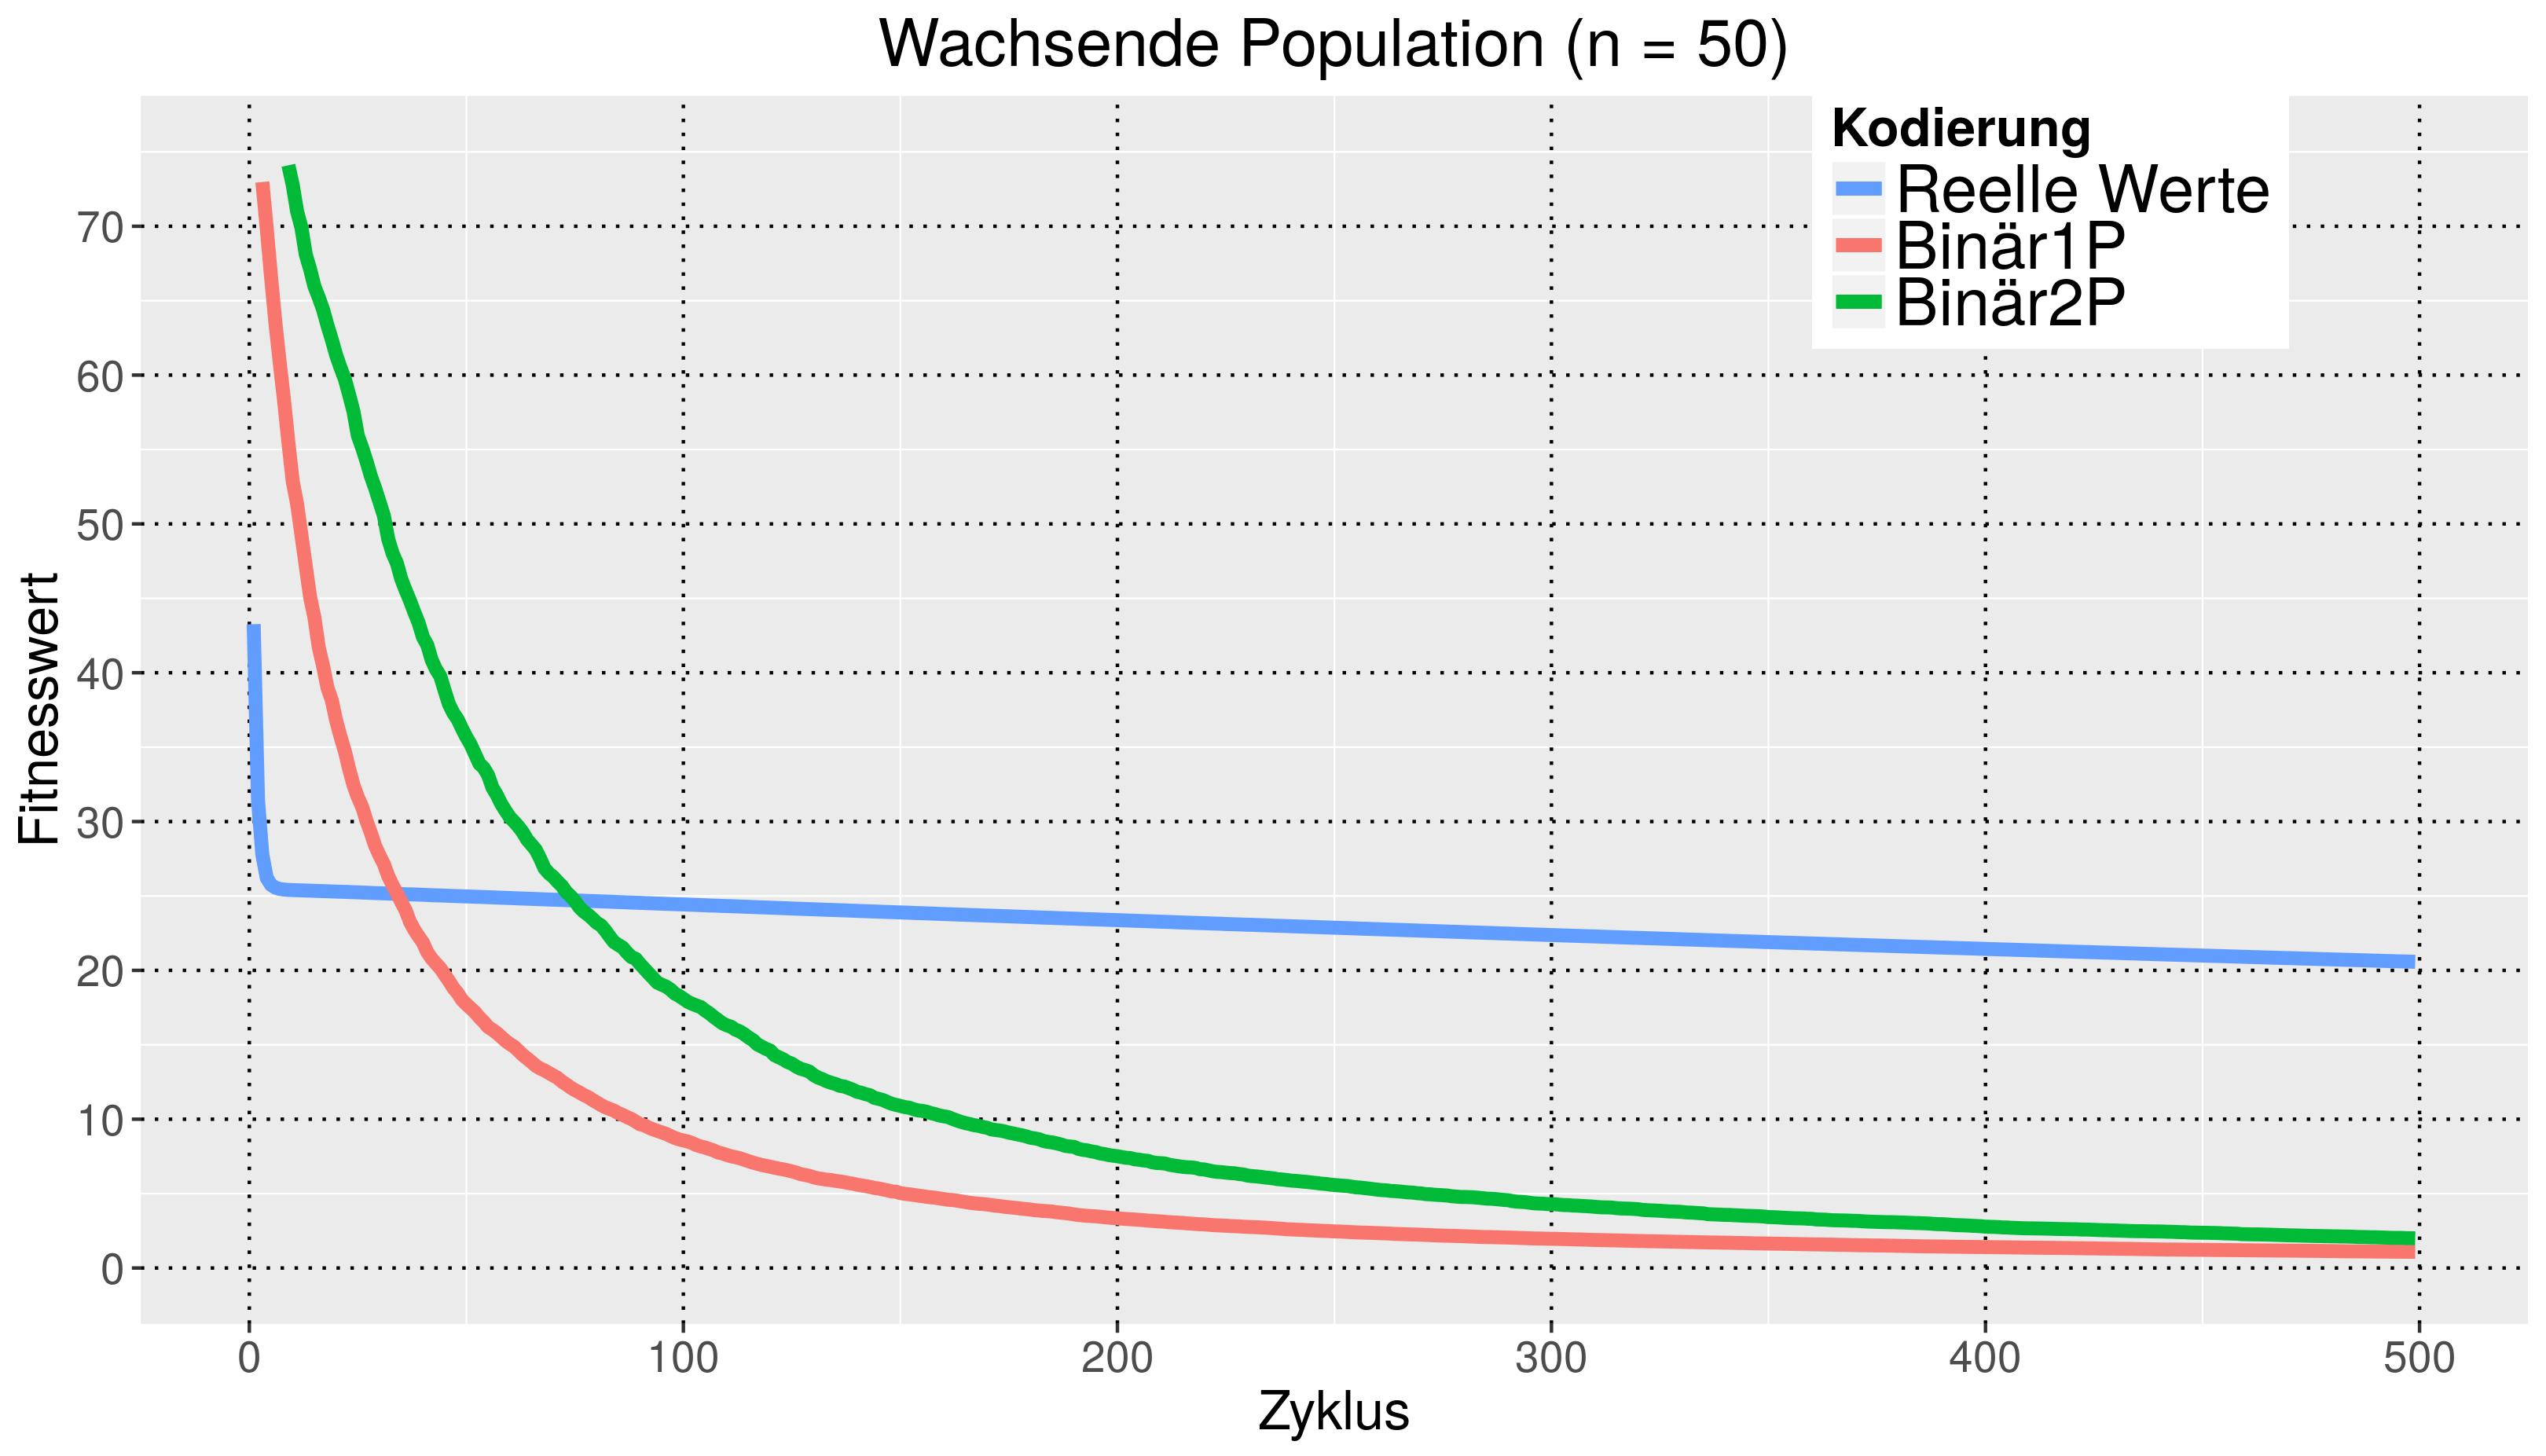
\includegraphics[width=\textwidth]{../abb2_growing.jpeg}
	\end{minipage}
	\caption*{Abb.2: Vergleich stabile und wachsende Population (n=50)} 
\end{figure}

Mit steigender Anzahl der Gene wird das globale Minimum immer verzögerter annähernd erreicht, wie in Abbildung 3 zu sehen ist.

Bei Betrachtung der Streuung der Individuen in Abbildung 4 ist auffällig, dass sich bei der reellen Kodierung das schlechteste und das beste Individuum sehr schnell annähern. Bei der binären Kodierung sind die Unterschiede etwas ausgeprägter. Es wird vermutet dass die Streuung maßgeblich für das Ergebnis verantwortlich ist, so dass die besseren Ergebnisse bei den binären Kodierungen aufgrund der größeren Streuung zwischen den Individuen zustande kommen.


\begin{figure}[H]
	\centering
	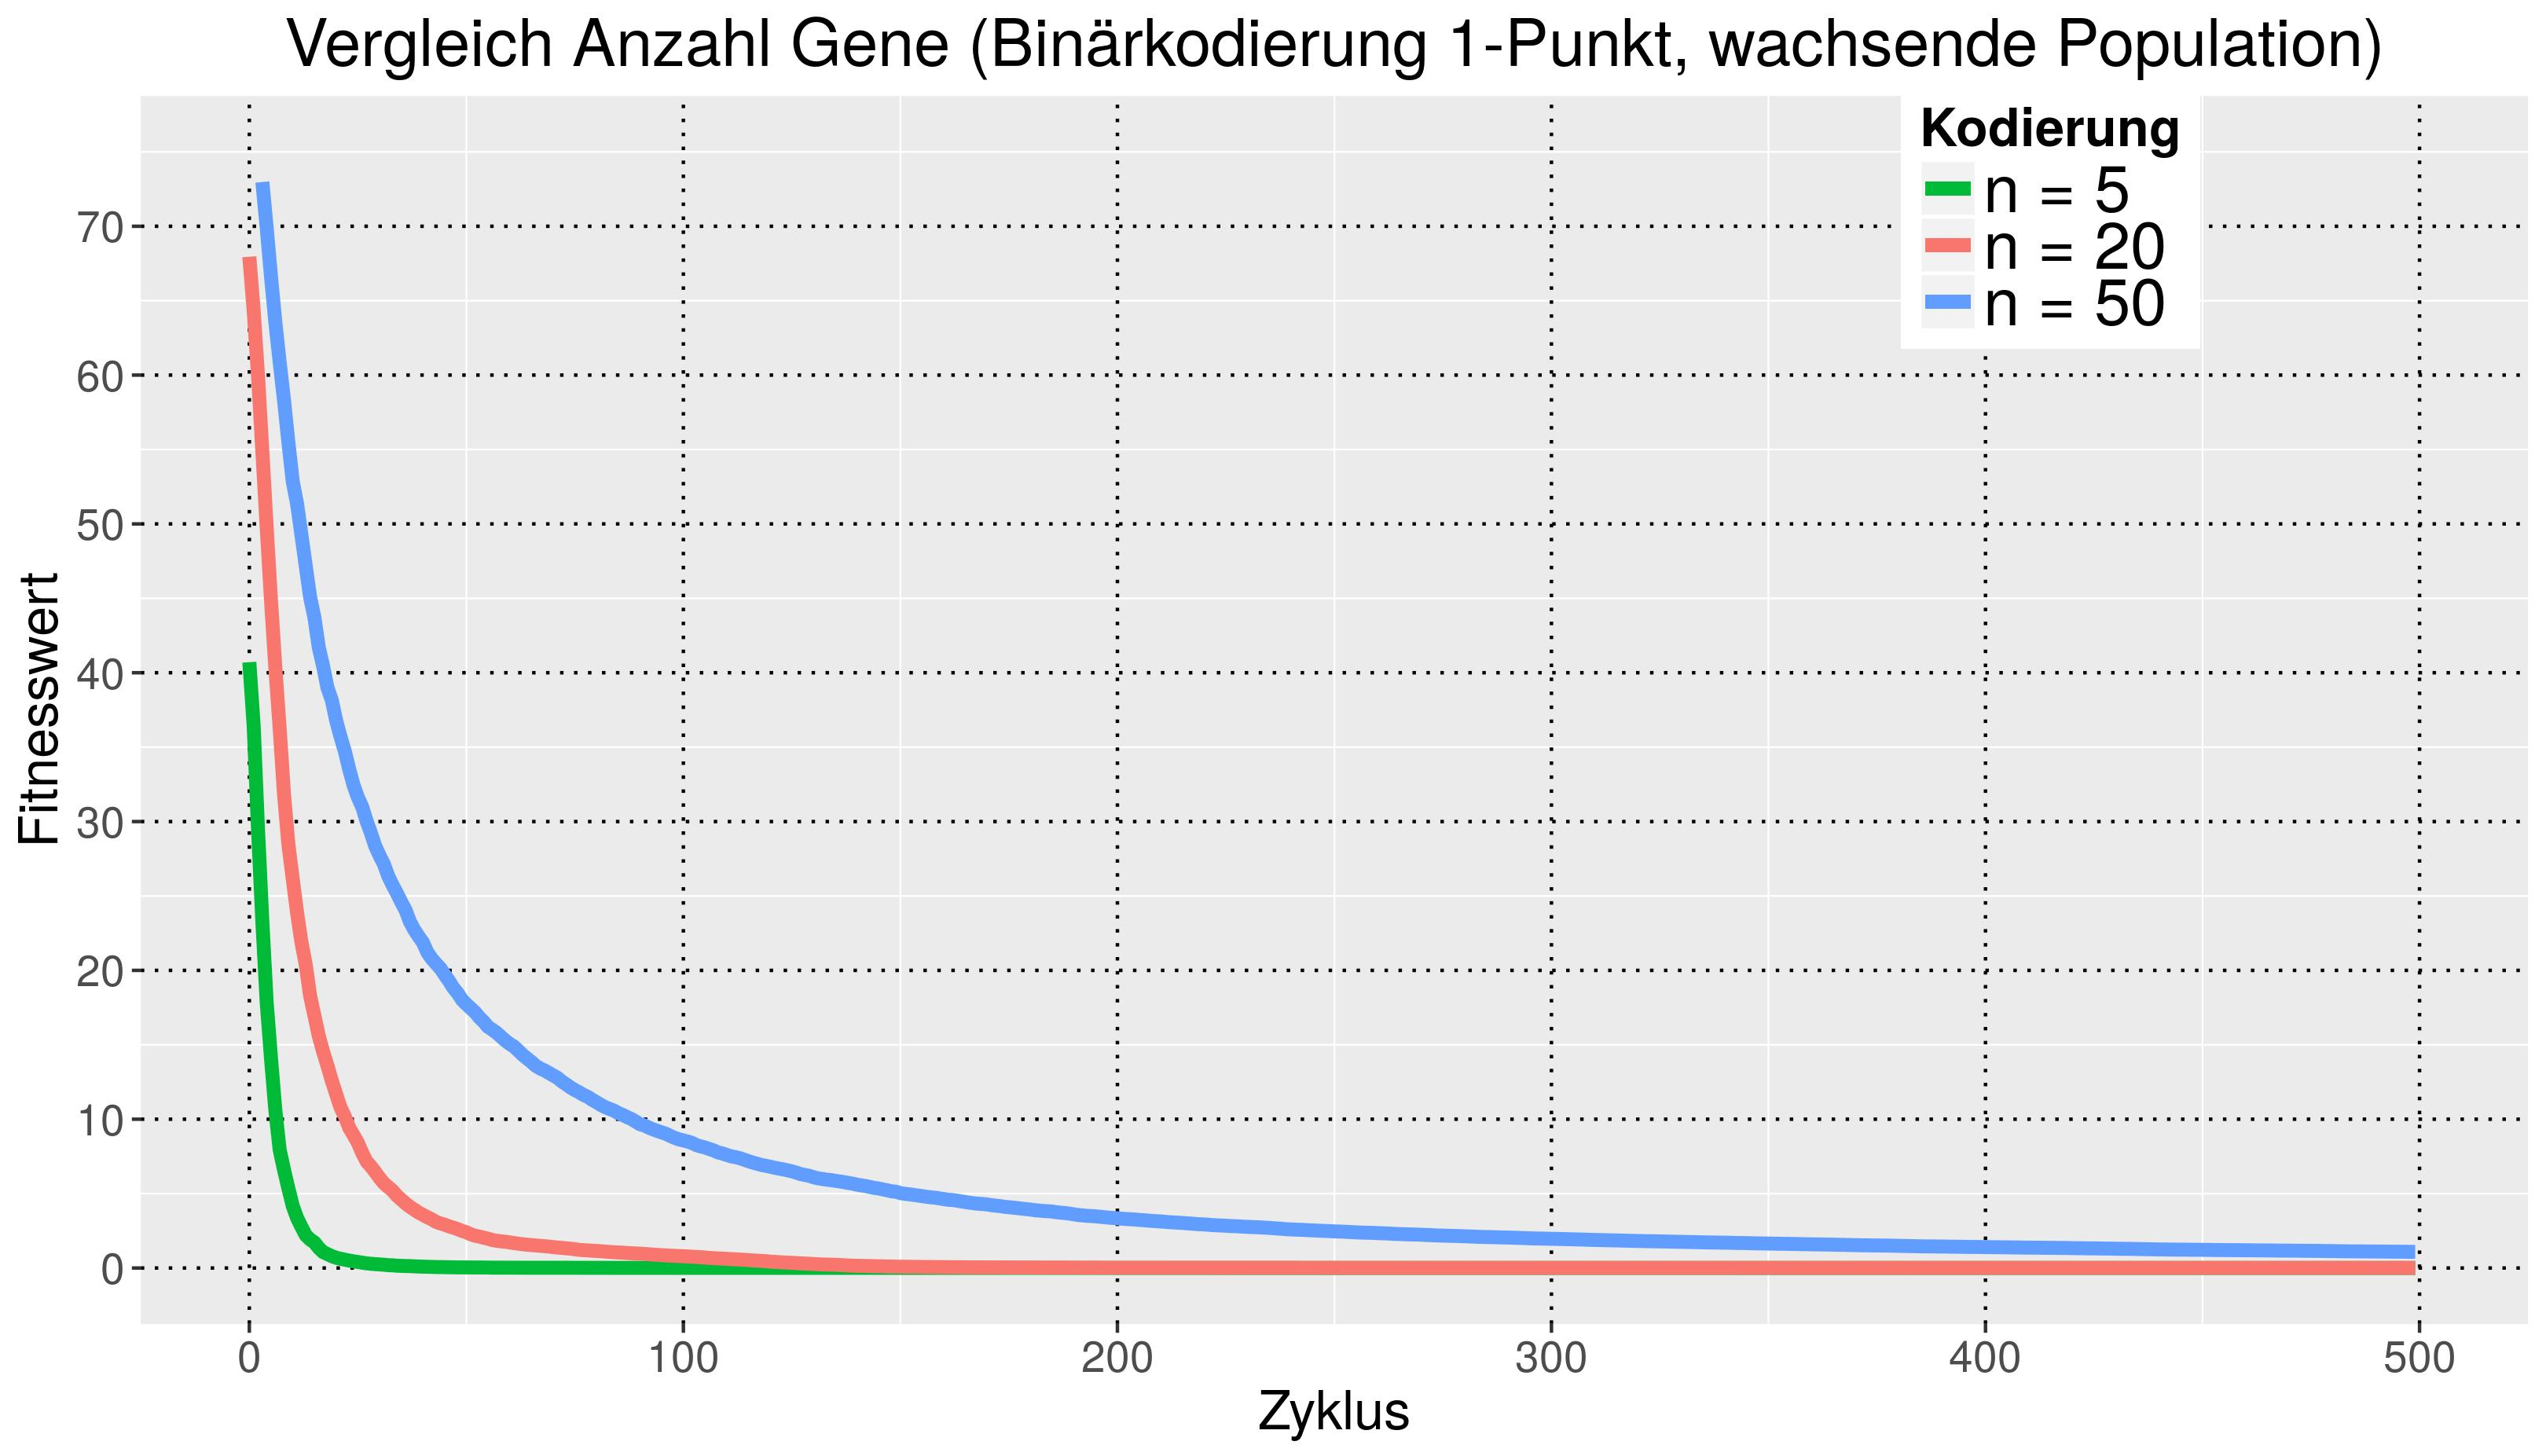
\includegraphics[width=0.7\textwidth]{../abb3_different_n.jpeg} 
	
	\caption*{Abb.3: Vergleich verschiedene Anzahl an Genen (Binärkodierung mit 1-Punkt-Rekombination, wachsende Population)} 
	\label{InputOutput}
\end{figure}


	\begin{figure}[H]
		\centering
		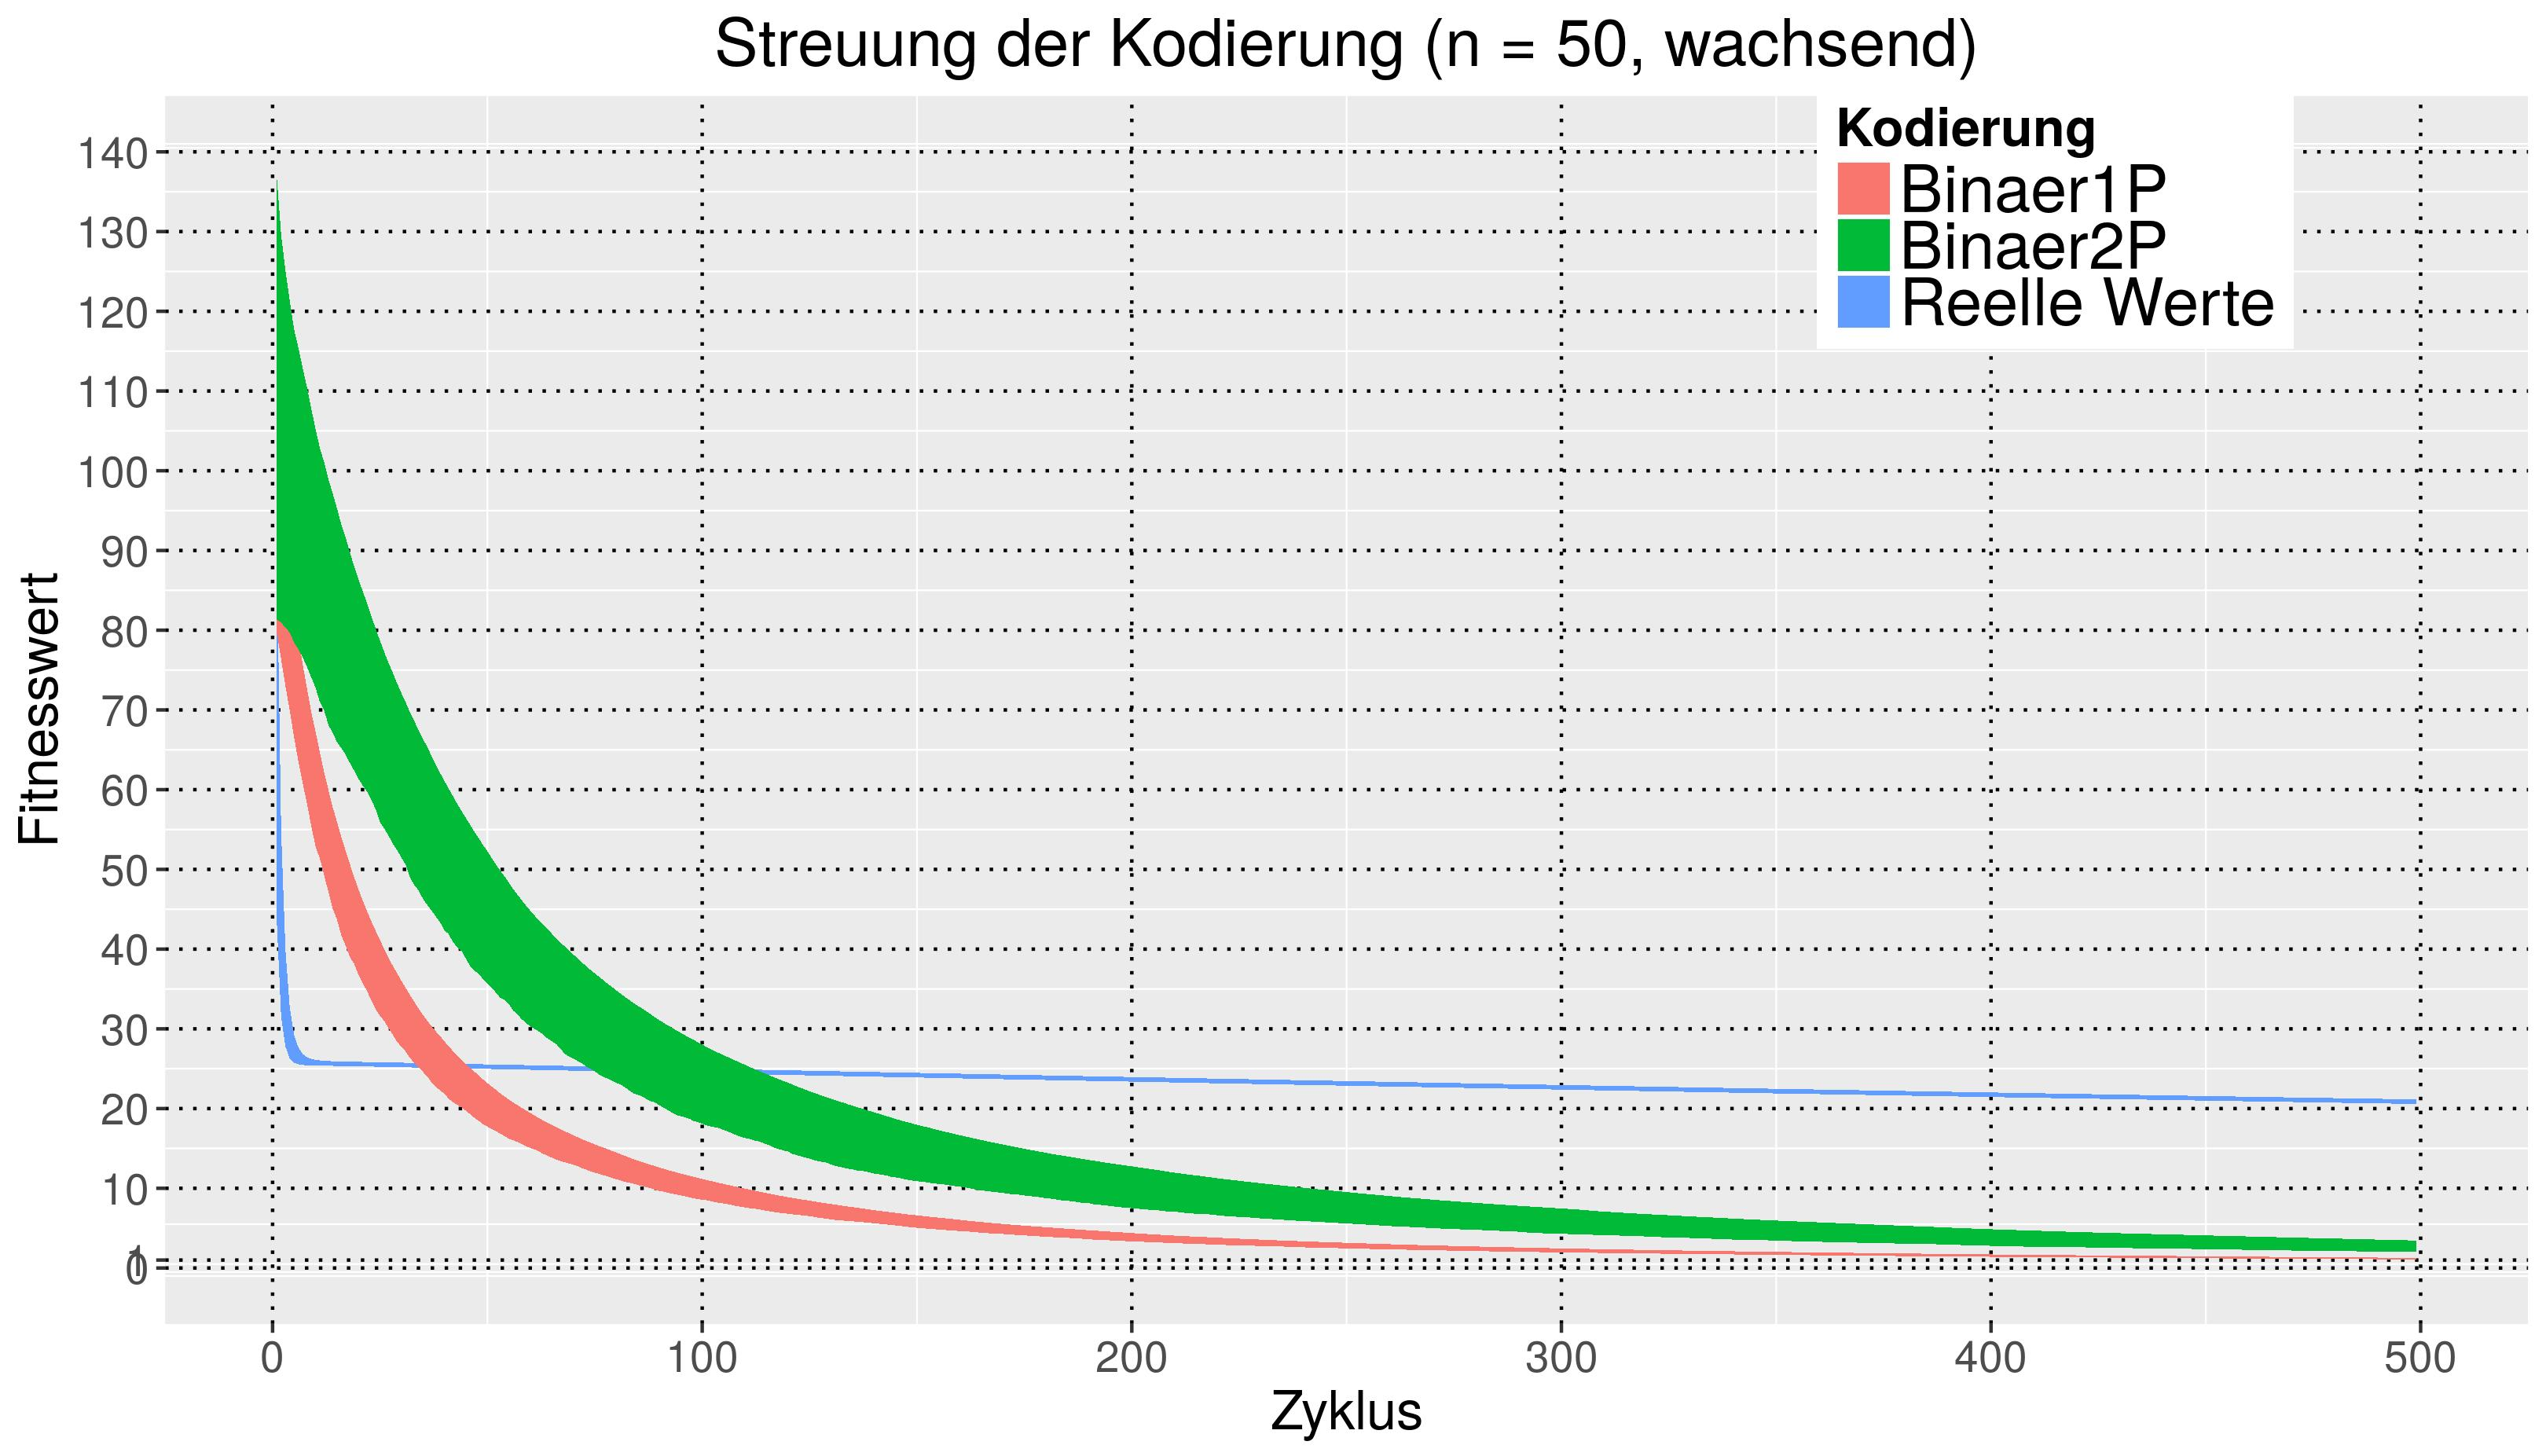
\includegraphics[width=0.7\textwidth]{../abb4_streuung.jpeg} 
		
		\caption*{Abb.4: Vergleich der Streuung innerhalb der Kodierungsarten (n = 50, wachsende Population)} 
		\label{InputOutput}
	\end{figure}

Im untersuchten Algorithmus liefert die reelle Kodierung generell schlechtere Ergebnisse. Ein Ansatzpunkt für bessere Ergebnisse  wäre, die Streuung der reell kodierten Individuen zu erhöhen. Durch die Anpassung  der weiteren Parameter des evolutionären Algorithmus sind bessere Ergebnisse zu erwarten. 

Ein Erklärungsansatz für den Unterschied zwischen reeller und binärer Kodierung stellt die spezielle Anforderung der Griewank-Funktion dar. Deren globales Minimum liegt exakt bei Null. Bei der reellen Kodierung kann entweder ein zufällig anfangs existierendes Individuum mit Allelen nah bei Null für das optimale Ergebnis sorgen. Außerdem ist dies über die Mutation möglich. 
Währenddessen bietet sich bei der Binärkodierung zusätzlich die Chance auf die Existenz eines solchen Individuums durch Rekombination von Elternpaaren, so dass sich ein Binärstrang ausschließlich aus Nullen ergeben kann.

	
	

	

	
	

	

	


	

	
	
	



%	\glsnogroupskiptrue
%	\printglossary[type=\acronymtype, title=Abkürzungsverzeichnis]
	
%	\listoffigures
%	\addcontentsline{toc}{chapter}{Abbildungsverzeichnis}
	
%	\lstlistoflistings
%	\addcontentsline{toc}{chapter}{Auflistungsverzeichnis}
	
%	\printbibliography 
%	\addcontentsline{toc}{chapter}{Literaturverzeichnis}
	
	
	%\begin{acronym}
	%	\acro{TCP}{Transmission Control Protocol}
	%	\acro{FTP}{File Transfer Protocol}
	%	\acro{IP}{Internet Protocol}
	%	\acro{DNS}{Domain Name Server}
	%	\acro{WWW}{World Wide Web}
%	\end{acronym}

\end{document}